%%%%%%%%%%%%%%%%%%%%%%%%%%%%%%%%%%%%%%%%%
% a0poster Portrait Poster
% LaTeX Template
% Version 1.0 (22/06/13)
%
% The a0poster class was created by:
% Gerlinde Kettl and Matthias Weiser (tex@kettl.de)
% 
% This template has been downloaded from:
% http://www.LaTeXTemplates.com
%
% License:
% CC BY-NC-SA 3.0 (http://creativecommons.org/licenses/by-nc-sa/3.0/)
%
%%%%%%%%%%%%%%%%%%%%%%%%%%%%%%%%%%%%%%%%%

%----------------------------------------------------------------------------------------
%	PACKAGES AND OTHER DOCUMENT CONFIGURATIONS
%----------------------------------------------------------------------------------------

\documentclass[a0,landscape,spanish]{a0poster}

\usepackage[spanish, mexico]{babel}
\selectlanguage{spanish}
\usepackage[utf8]{inputenc}
\usepackage{float}
\usepackage{mathrsfs}
\usepackage{mathtools}
\usepackage{ragged2e}
\usepackage{multicol} % This is so we can have multiple columns of text side-by-side
\columnsep=100pt % This is the amount of white space between the columns in the poster
\columnseprule=3pt % This is the thickness of the black line between the columns in the poster

\usepackage[svgnames]{xcolor} % Specify colors by their 'svgnames', for a full list of all colors available see here: http://www.latextemplates.com/svgnames-colors

\usepackage{times} % Use the times font
%\usepackage{palatino} % Uncomment to use the Palatino font

\usepackage{graphicx} % Required for including images
\graphicspath{{figures/}} % Location of the graphics files
\usepackage{booktabs} % Top and bottom rules for table
\usepackage[font=small,labelfont=bf]{caption} % Required for specifying captions to tables and figures
\usepackage{amsfonts, amsmath, amsthm, amssymb} % For math fonts, symbols and environments
\usepackage{wrapfig} % Allows wrapping text around tables and figures

\usepackage{titlesec}
\titlespacing*{\section}{0pt}{0.85\baselineskip}{\baselineskip}

\begin{document}

%----------------------------------------------------------------------------------------
%	POSTER HEADER 
%----------------------------------------------------------------------------------------

% The header is divided into two boxes:
% The first is 75% wide and houses the title, subtitle, names, university/organization and contact information
% The second is 25% wide and houses a logo for your university/organization or a photo of you
% The widths of these boxes can be easily edited to accommodate your content as you see fit

\begin{minipage}[b]{0.75\linewidth}
\veryHuge \color{NavyBlue} \textbf{MULTI-OBJECTIVE OPTIMIZATION BASED ON PARAMETER TUNING OF CLAHE TO ACHIEVE DIFFERENT CONTRAST LEVELS IN MEDICAL IMAGES} \color{Black}\\[2ex] % Title
%\Huge\textit{An Exploration of Complexity}\\[2cm] % Subtitle
\huge \textbf{Luis G. Moré, Marcos Brizuela, José L. Vázquez, Diego Pinto, Horacio Legal}\\[0.5cm] % Author(s)
\huge Facultad Politécnica - Universidad Nacional de Asunción% University/organization
%\Large \texttt{john@LaTeXTemplates.com} --- 1 (000) 111 1111\\
\end{minipage}
%
\begin{minipage}[b]{0.25\linewidth}

\includegraphics[width=19cm]{photo.jpg}\\
\end{minipage}

%\vspace{0.5cm} % A bit of extra whitespace between the header and poster content

%----------------------------------------------------------------------------------------

\begin{multicols}{3} % This is how many columns your poster will be broken into, a portrait poster is generally split into 2 columns

%----------------------------------------------------------------------------------------
%	ABSTRACT
%----------------------------------------------------------------------------------------

\color{Navy} % Navy color for the abstract


%----------------------------------------------------------------------------------------
%	INTRODUCTION
%----------------------------------------------------------------------------------------

\color{SaddleBrown} % SaddleBrown color for the introduction

\section*{Motivación}

Las imágenes con problemas de contraste necesitan de transformaciones que logren que las mismas sean útiles para análisis posteriores u otras aplicaciones. Ésto es particularmente crítico en imágenes médicas y biométricas, en las que se necesita preservar los detalles finos para mantener la información sensible contenida en éstas, a la vez que se logre resaltar detalles difíciles de percibir. Es necesario lograr la mejora del contraste sin degradar la calidad de la imagen que se transforma.
\color{Black} % DarkSlateGray color for the rest of the content
\section*{Conceptos Básicos}

\begin{enumerate}
\item{\it \textbf{CLAHE}}: Para mejorar el contraste de una imagen, se ha escogido el algoritmo Contrast Limited Adaptive Histogram Equalization ($CLAHE$), que es un algoritmo de mejora de contraste local basado en la división de la imagen en bloques y la ecualización del histograma de cada bloque de forma independiente, propuesto en \cite{Zuiderveld:1994:CLA:180895.180940}. %$CLAHE$ ha demostrado tener buenos resultados principalmente en el procesamiento de imágenes con bajo contraste \cite{balvant2011} e imágenes médicas \cite{saikat2011,shelda2013}, debido a que en este tipo de imagen se priorizan los detalles locales de una imagen.


\item {\it \textbf{Entropía}}: Es un coeficiente asociado con el aumento de la información contenida en una imagen como consecuencia del aprovechamiento de los niveles de gris disponibles para la representación de la misma. Al maximizar la Entropía de la imagen, también se aumenta el contraste que posee. 

\item {\it \textbf{Índice de Similitud Estructural}}: El Índice de Similitud Estructural ($SSIM$ por sus siglas en inglés Structural SIMilarity Index) es un coeficiente que permite evaluar los cambios producidos en la información estructural de una imagen luego de haber sufrido alguna modificación. Esta métrica da como resultado una buena medida de la distorsión o degradación estructural de la imagen que puede ser producida por cualquier algoritmo de mejora de imágenes.

\item{\it \textbf{PSO}}: La \textit{Optimización de Enjambre de Partículas} es un algoritmo metaheurístico de optimización, capaz de explorar un amplio espacio de búsqueda. Las partículas almacenan la mejor solución que encuentran durante la búsqueda, y el enjambre almacena la mejor solución global. Las partículas se van moviendo hacia la solución más óptima a su propio ritmo. El enjambre termina de moverse cuando encuentran la mejor solución o una muy cercana a ella debido a que se ha llegado a un criterio de parada.

\begin{center}\vspace{0.5cm}
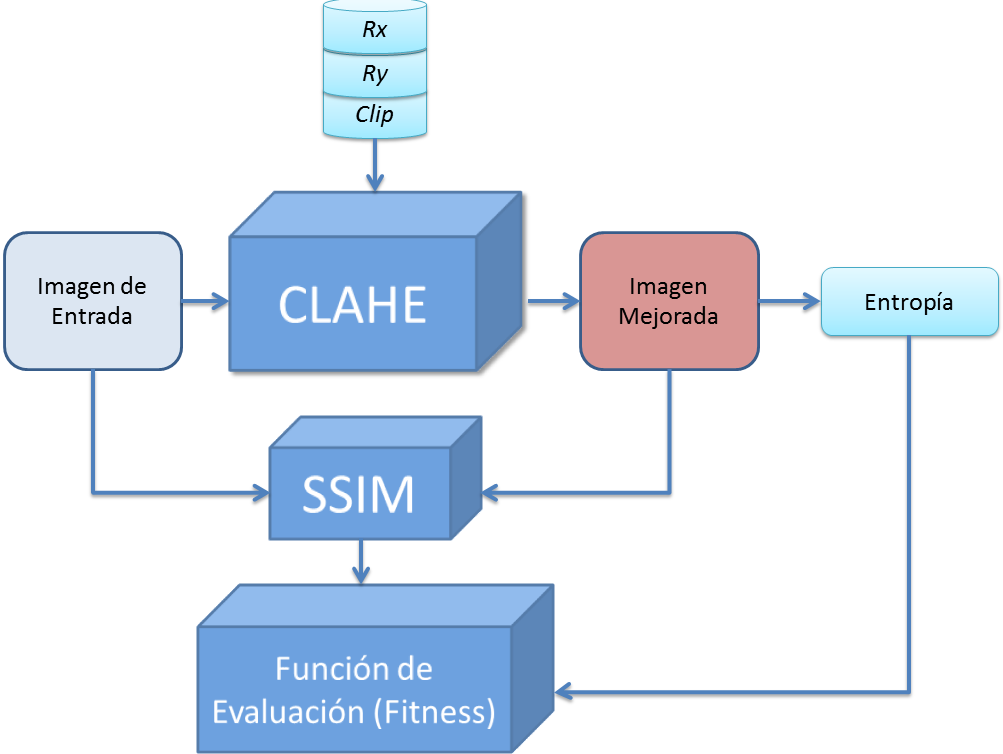
\includegraphics[width=0.55\linewidth]{particula_clahe}
\captionof{figure}{\color{Green} Esquema de evaluación de cada partícula durante la búsqueda de la solución.}
\label{esquema_evaluacion_pso_clahe}
\end{center}\vspace{0.5cm}

\end{enumerate}

\section*{Formulación}

Dadas la imagen de entrada $I$ y el algoritmo $CLAHE$, se desea calcular la mejor solución $f(T)$ que maximice:

\begin{equation*}\label{eq:fitness}
    f(T) = f_1(T) \times f_2(I,T)
\end{equation*}

donde:
\begin{itemize}
%\item $\overrightarrow{x}=(\mathcal{R}_x, \mathcal{R}_y, \mathcal{C})$, donde $\mathcal{R}_x$ y $\mathcal{R}_y$ conforman la región contextual y $\mathscr{C}$ es el Clip Limit.
\item $f_{1}(T)=\frac{\mathscr{H}(T)}{log_{2}L}$ es la Entropía normalizada de la imagen $T$, siendo $T$ la imagen mejorada por $CLAHE$.
\item $f_{2}(I,T)=SSIM(I,T)$ es el Índice de Similitud Estructural.

\item $I$ = Imagen Original.
\item $T$ = Imagen con contraste mejorado.
\end{itemize}

\color{DarkSlateGray} % Set the color back to DarkSlateGray for the rest of the content


\section*{Propuesta}

La propuesta consiste en utilizar un algoritmo de mejora de contraste por bloques (Contrast Limited Adaptive Histogram Equalization - $CLAHE$) el cual posee ciertos parámetros de entrada que necesitan de optimización, de manera a lograr maximizar la mejora del contraste, minimizando la distorsión introducida. Para encontrar éstos parámetros se utiliza una metaheurística (Particle Swarm Optimization - $PSO$) que permite realizar una búsqueda eficiente, además de que permite evaluar los resultados obtenidos durante la exploración utilizando una función de adaptación $f(T)$ , que está compuesta por dos métricas (Entropía e Índice de Similitud Estructural) que logran medir cuánta mejora en el contraste se logró, y cuánta distorsión se introdujo, respectivamente. En la Figura \ref{esquema_evaluacion_pso_clahe} se muestra la interacción entre las partículas de $PSO$, el algoritmo de $CLAHE$, y cómo se efectúa la evaluación de resultados.


%\section*{Propuesta}
%    \begin{itemize}\justifying
%    \item Para optimizar $f(T)$ se utiliza la Optimización de Enjambre de Partículas, el cual consiste  en un algoritmo metaheurístico de optimización, capaz de explorar un amplio espacio de búsqueda.
%    \item Evaluar la calidad de las soluciones posibles de tal forma a que la imagen resultante posea la mayor cantidad de información posible y el menor grado de distorsión.
%    \item Para ello, se maximizará la Entropía de la imagen y se maximizará el Índice de Similitud Estructural $SSIM$.
%    \end{itemize}


%\begin{figure}[h!]\centering
%    \includegraphics[height=6.5cm]{flujo}
%\caption{Diagrama de flujo básico de $PSO$.}
%\end{figure}


%----------------------------------------------------------------------------------------
%	MATERIALS AND METHODS
%----------------------------------------------------------------------------------------
\color{Black} % DarkSlateGray color for the rest of the content
\section*{Resultados}

Para validar los resultados obtenidos por $PSO-CLAHE$, se implementó el enfoque propuesto por Byong Seok Min \cite{byong2013}. Los resultados se muestran en las Figuras \ref{fig:resultado_chest}, \ref{fig:resultado_lenna} y \ref{fig:resultado_iris} para la comparación visual, y en la Figura \ref{fig:resultado_metricas} para la comparación de resultados de métricas:

\begin{figure}[H]
    \centering
    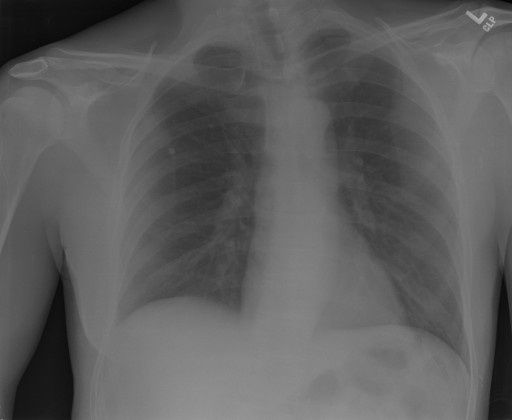
\includegraphics[width=11cm]{chestoriginal}
    \hspace{1pt}
    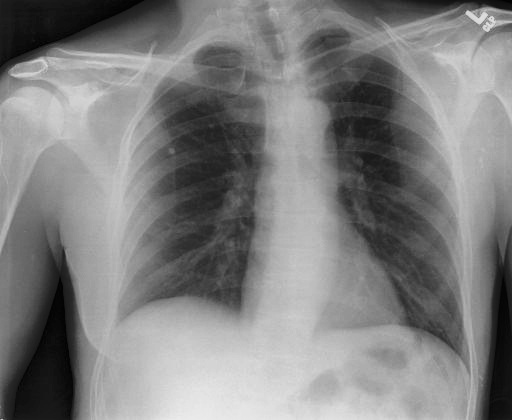
\includegraphics[width=11cm]{chestclahe}
    \hspace{1pt}
    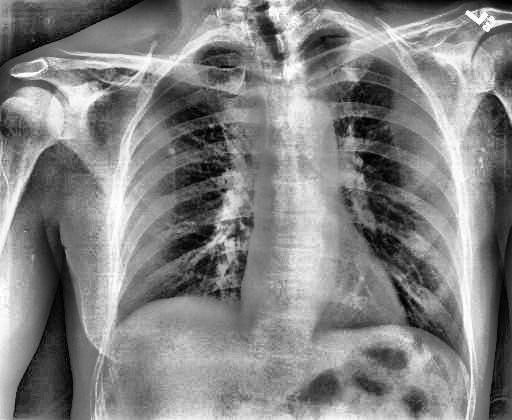
\includegraphics[width=11cm]{chestclahelicen}
  

  \caption{\textbf{Imagen de radiografía de tórax.} \\
(a) Original. (b) $PSO-CLAHE$. $f(T)$=0,8224 (c) Byong. $f(T)$=0,496}
\label{fig:resultado_chest}
\end{figure}

\begin{figure}[H]
\centering
\captionsetup{justification=centering}
 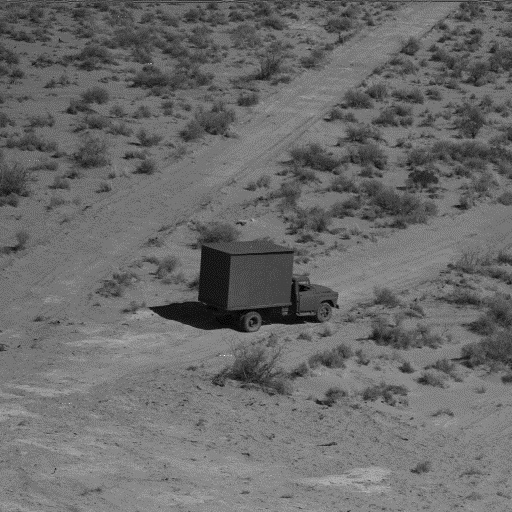
\includegraphics[width=10.5cm]{Camionoriginal.jpg}
 \hspace{0.1pt}
 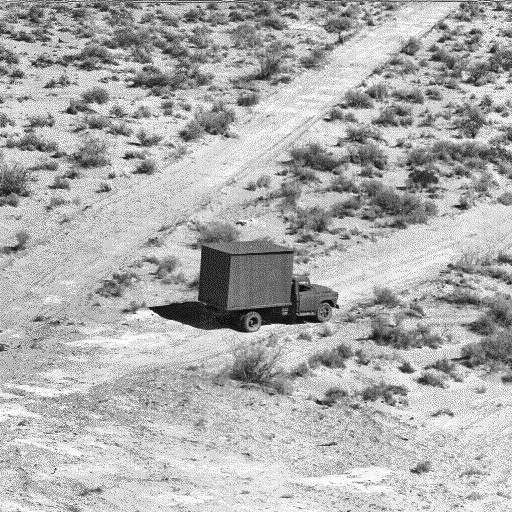
\includegraphics[width=10.5cm]{Camionclahe.jpg}
 \hspace{0.1pt}
 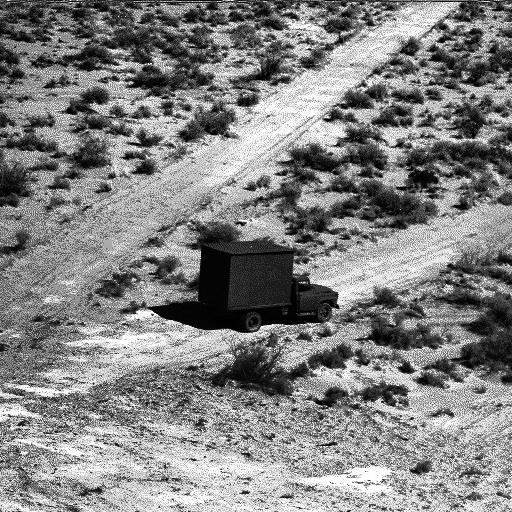
\includegraphics[width=10.5cm]{Camionclahelicen.jpg}
 \caption{\textbf{Comparación de resultados para una imagen miscelánea.} \\
(a) Original. (b) $PSO-CLAHE$. $f(T)$=0,7607 (c) Byong. $f(T)$=0,4690}
\label{fig:resultado_lenna}
\end{figure}

\begin{figure}[H]
    \centering
    \captionsetup{justification=centering}
    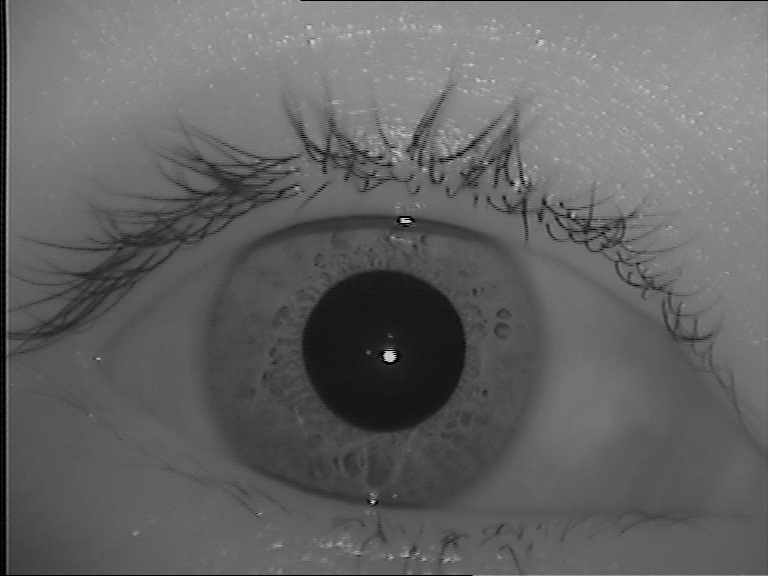
\includegraphics[width=11cm]{retina2original.jpg}
    \hspace{1pt}
    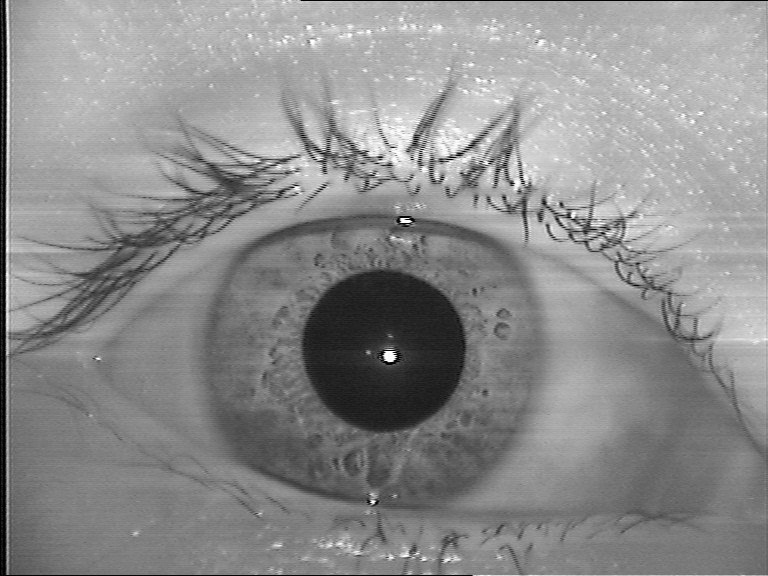
\includegraphics[width=11cm]{retina2clahe.jpg}
    \hspace{1pt}
    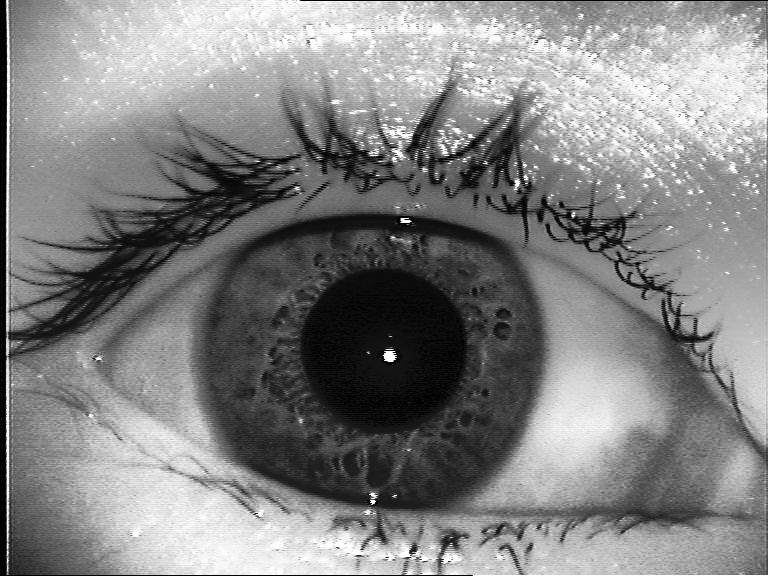
\includegraphics[width=11cm]{retina2clahelicen.jpg}
  
  \caption{\textbf{Comparación de resultados para una imagen biométrica.} \\
(a) Original. (b) $PSO-CLAHE$. $f(T)$=0,7683 (c) Byong. $f(T)$=0,5356}
\label{fig:resultado_iris}
\end{figure}
\begin{figure}[H]
    \centering
    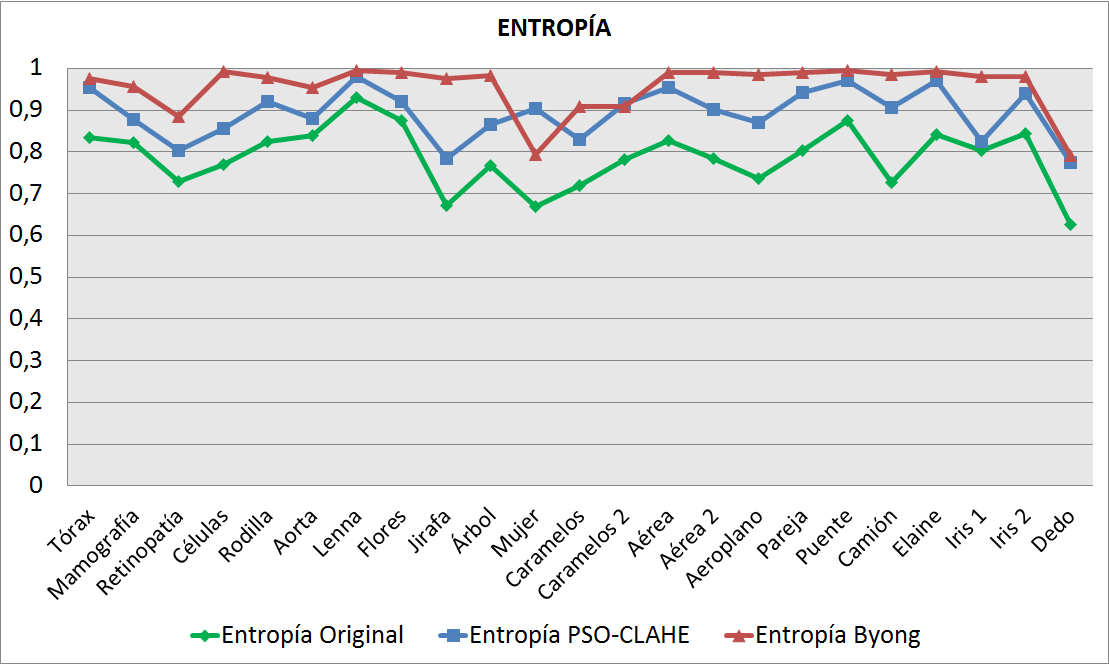
\includegraphics[height=8cm]{grafica1}
    \hspace{1pt}
    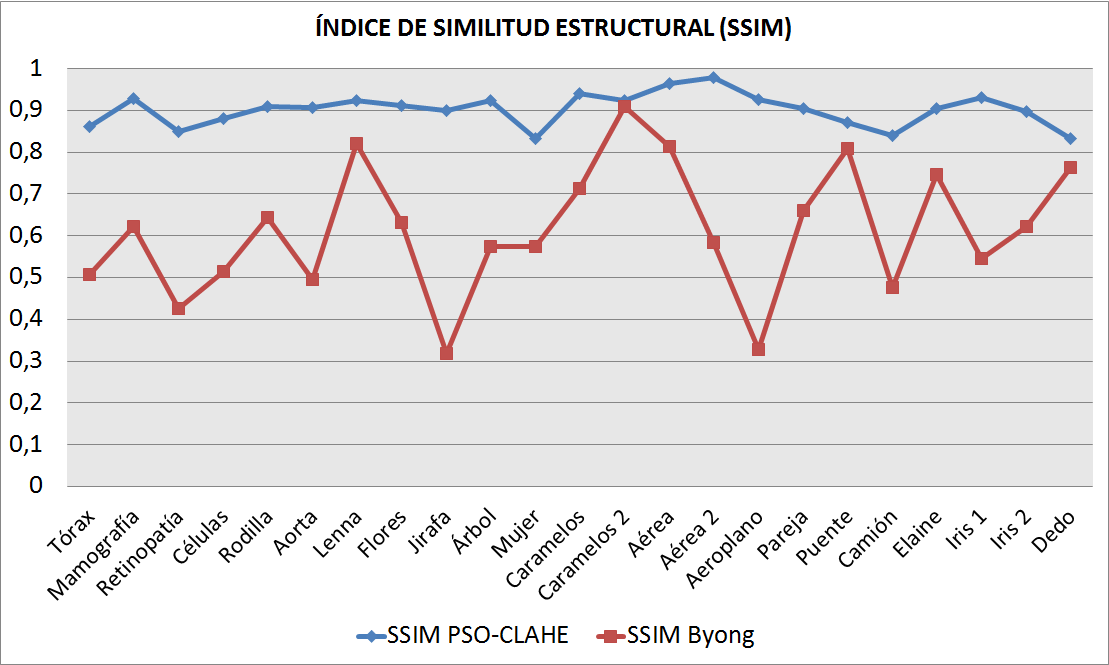
\includegraphics[height=8cm]{grafica2}
    \hspace{1pt}
    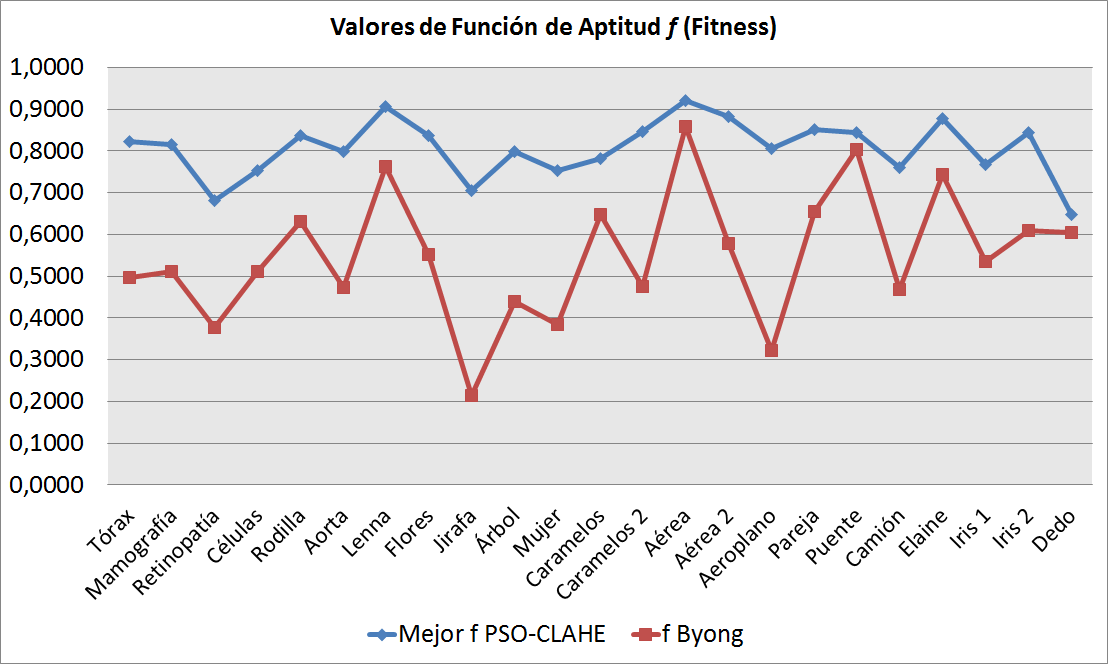
\includegraphics[height=8cm]{grafica3}
    \hspace{1pt}

  
  \caption{(a) Comparación de Entropía entre resultados para $PSO-CLAHE$ y Byong (b) Compararación de $SSIM$ entre $PSO-CLAHE$ y Byong (c) Comparación de $f(T)$ entre $PSO-CLAHE$ y Byong.}
\label{fig:resultado_metricas}
\end{figure}


%------------------------------------------------


\color{DarkSlateGray} % Set the color back to DarkSlateGray for the rest of the content


\section*{Conclusiones}

\begin{itemize} \justifying


\item Los resultados de todas las imágenes para $PSO-CLAHE$ muestran una clara mejora en el contraste, manteniendo la apariencia natural de las mismas.

%\item $PSO-CLAHE$ puede recorrer el espacio de búsqueda más ampliamente que la propuesta de Byong, debido a que Byong acota el dicho espacio de búsqueda y $PSO-CLAHE$ toma el espacio completo. 


\item El aporte más importante del trabajo es la utilización efectiva  de $CLAHE$, $PSO$ y unas métricas de evaluación de resultados (Entropía y $SSIM$) que permiten la mejora del constraste en imágenes en escala de grises, sin introducir una distorsión apreciable en las mismas. 


\end{itemize} 


%----------------------------------------------------------------------------------------
%	RESULTS 
%----------------------------------------------------------------------------------------

\section*{Trabajos Futuros}


\begin{itemize}\justifying

\item Utilizar una implementación multi-objetivo de $PSO$, de manera a introducir objetivos que se consideren adecuados para la mejora del contraste.

%\item Encontrar otros casos prácticos de manera a validar los resultados obtenidos por $PSO-CLAHE$.

\item Realizar modificaciones al algoritmo de $CLAHE$ de manera a que se tengan en cuenta múltiples ventanas de tamaños variables durante la optimización con $PSO$.

\item Realizar una implementación de $PSO-CLAHE$, o una combinación de metaheurística con una técnica de mejora del contraste adaptada para imágenes a color.
\end{itemize} 

%----------------------------------------------------------------------------------------
%	CONCLUSIONS
%----------------------------------------------------------------------------------------


%----------------------------------------------------------------------------------------
%	FORTHCOMING RESEARCH
%----------------------------------------------------------------------------------------

 %----------------------------------------------------------------------------------------
%	REFERENCES
%----------------------------------------------------------------------------------------

%\nocite{*} % Print all references regardless of whether they were cited in the poster or not
\bibliographystyle{unsrt}
\bibliography{sample.bib}

%----------------------------------------------------------------------------------------
%	ACKNOWLEDGEMENTS
%----------------------------------------------------------------------------------------

%\section*{Reconocimientos}

%Etiam fermentum, arcu ut gravida fringilla, dolor arcu laoreet justo, ut imperdiet urna arcu a arcu. Donec nec ante a dui tempus consectetur. Cras nisi turpis, dapibus sit amet mattis sed, laoreet.

%----------------------------------------------------------------------------------------

\end{multicols}
\end{document}